% ~ 6 pages
\chapter{Theoretical Background}
\label{sec:theory}

\section{The Standard Model}

\section{The Weak \& Strong Interaction}

\section{$\tau$-Leptons}

\begin{figure}[ht]
  \begin{subfigure}[b]{0.47\textwidth}
    \centering
    \begin{overpic}{./figures/theory/tau_branching_pie_chart.pdf}
      \put (34, 83) {$\pi^- \nu_\tau$}
      \put (-1, 45) {$\pi^- \pi^0 \nu_\tau$}
      \put (19, 8) {$\pi^- 2 \pi^0 \nu_\tau$}
      \put (44.5, 2) {$2 \pi^- \pi^+ \nu_\tau$}
      \put (69, 6) {$2 \pi^- \pi^+ \pi^0 \nu_\tau$}
      \put (80, 15) {other}
    \end{overpic}
    \caption{Tau branching ratios\cite{pdg}. Fix wonky percentages for hadronic
      modes.}
    \label{fig:tau_branching_ratios}
  \end{subfigure}\hfill
  \begin{subfigure}[b]{0.47\textwidth}
    \centering
    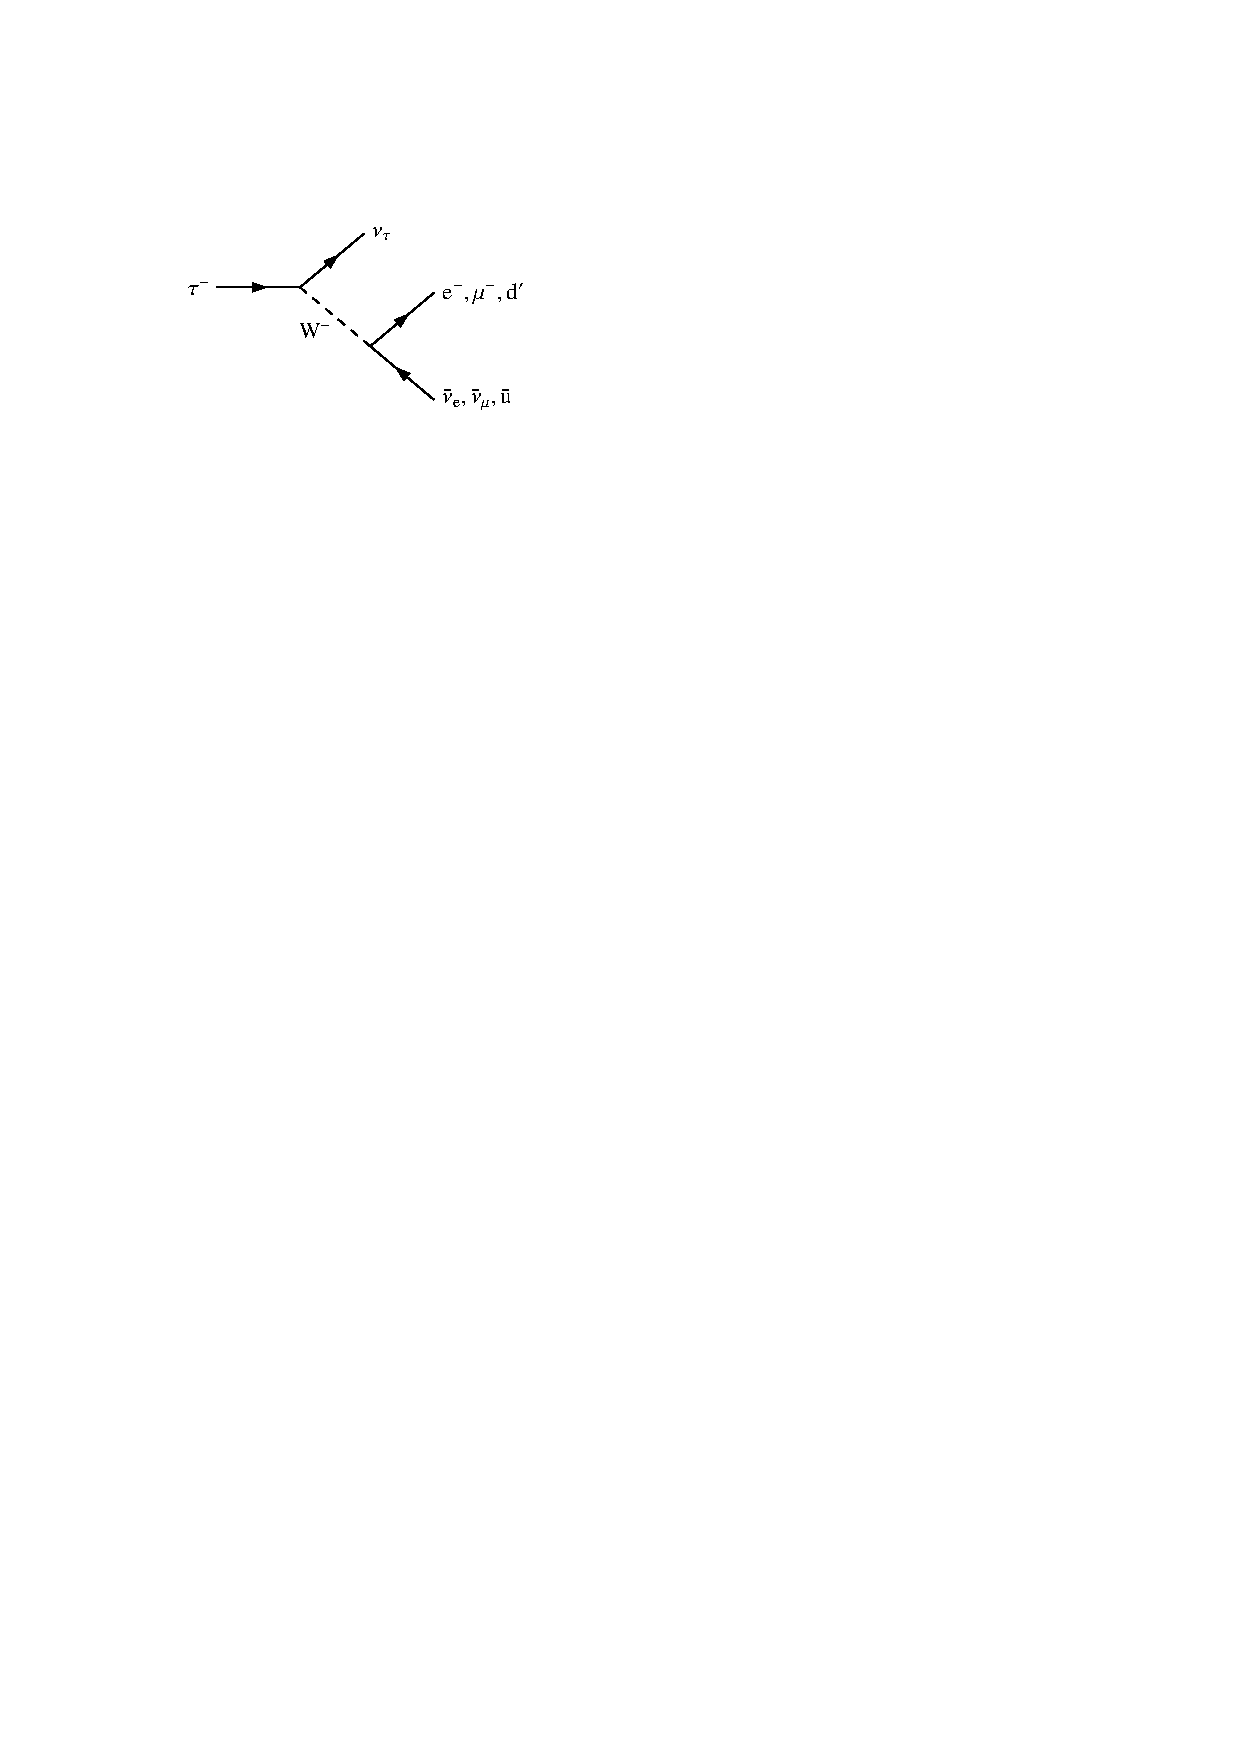
\includegraphics{./figures/theory/tau_decay_feynman.pdf}
    \caption{Feynman Diagram. Strangeness production is Cabibbo suppressed by a
      factor of $\sin^2\theta_\mathrm{c} / \cos^2\theta_\mathrm{c} \approx
      \frac{1}{20}$. Ignoring phase space considerations the tau decays to
      $\frac{1}{5}$ into electron or muon and corresponding antineutrino or into
      a down anti-up quark pair (3 colours). W-boson should be wiggly line.}
  \end{subfigure}
  \caption{Weak decay of the tau-lepton}
\end{figure}

\begin{itemize}
\item Discovery at SPEAR in 1975 [Check Citation]\cite{perl}
\item $m_\tau = \SI{1776.86 +- 0.12}{\mega\electronvolt}$ \cite{pdg}
\item Tau more than twelve times heavier than pions \textrightarrow can decay
  into quark-antiquark pairs (strangeness production cabbibo suppressed)
\item 5 possible weak decay modes: electron (20\%), muon (20\%), ud (3 times
  20\% due to 3 color charges) -- ignoring phase space
\item unit charge \textrightarrow decays into odd number of charged particles
  (prong definition)
\end{itemize}

% ----------------------- FIRST DRAFT ---------------------- %
\begin{itemize}

\item The Standard Model
  \begin{itemize}
  \item Features \& Successes

  \item Challenges (neutrino masses, dark matter, matter-antimatter asymmetry,
    gravitation, number of parameters, hierarchy problem, \ldots)

  \item Beyond the Standard Model (SUSY -- preferred coupling to down-type
    fermions for large $\tan\beta$ \textrightarrow $\tau$-leptons)
  \end{itemize}

\item Weak Interaction
\begin{itemize}
\item Can be kept very short. Only whats necessary to understand Tau-ID
\end{itemize}

\item Strong Interaction
\begin{itemize}
\item Can be kept very short. Only whats necessary to understand Tau-ID
\item Confinement \& Hadronization
\item Quark \& Gluon initiated jets
\end{itemize}

\item $\tau$-Leptons
\begin{itemize}
\item Discovery

\item Properties (mass \textrightarrow lep \& had, mean life time
  \textrightarrow no direct detection)

\item Hadronically Decaying $\tau$-Leptons
  \begin{itemize}
  \item Feynman Diagram, Decay Modes (interm. resonances) \& Branching Ratios
    (pie chart like in: \url{https://www.lhc-ilc.physik.uni-bonn.de/ergebnisse/dateien/t00000078.pdf?c=t&id=78}
    on p.\ 25)
  \item Detector signature ($\pi^0$ ($\gamma \gamma$ / $\mathrm{e}^+
    \mathrm{e}^- \gamma$), $\pi^\pm$ ($\mathrm{K}^\pm$), $\nu_\tau$,
    conversions)
  \item Jets faking taus
  \end{itemize}

\item $\tau$ Physics
  \begin{itemize}
  \item $\mathrm{Z} \rightarrow \tau \tau$ (background for H$\tau \tau$ and
    useful for performance measurements using tag-and-probe -- semileptonic
    decays)

  \item $\mathrm{H} \rightarrow \tau \tau$ (one of two channels to measure
    the fermionic coupling -- $b \bar{b}$ plagued by multijet background,
    Higgs CP)

  \item MSSM Higgs (potentially high branching fraction to $\tau$-leptons)

  \item $\mathrm{Z}^\prime$ could preferentially decay into third-generation
    fermions (lepton universality not required).

  \item $\mathrm{W}^\prime$ models with preferential coupling to third-gen.

  \item SUSY with $\tau$ \textrightarrow long decay chains
  \end{itemize}
\end{itemize}
\end{itemize}

% -----------------------------???-------------------------- %

\begin{itemize}
\item Tau lepton

\item Weak \& strong interaction (?)
  \begin{itemize}
  \item Cross section plot multijet (large cross section) vs.
    electroweak interaction (small)
  \item \url{http://www.hep.ph.ic.ac.uk/~wstirlin/plots/plots.html}
  \item Quark vs Gluon jets: \url{http://jets.physics.harvard.edu/qvg/}
    Because of different colour interaction and hadronization, gluon jets are
    wider, with higher multiplicity and have a more uniform energy
    fragmentation, while quark jets are more likely to produce narrow jets with
    hard constituents that carry a significant fraction of the energy.
  \end{itemize}

\item Tau decay modes \& branching fractions
  \begin{itemize}
  \item Hadronic decays not containing pions but kaons etc.
  \end{itemize}

\item Intermediate resonances $a$, $\rho$

\item Jets (anti-$k_\mathrm{T}$)

\end{itemize}

%%% Local Variables:
%%% mode: latex
%%% TeX-master: "mythesis"
%%% End:
